\documentclass[10pt]{beamer}

\usetheme{metropolis}
\usepackage{appendixnumberbeamer}

\usepackage{booktabs}							% You should use \toprule, \midrule, and \bottomrule in tables
\usepackage{tabularx}								% Helps with scaling the table to content
\usepackage{natbib}

\usepackage{algorithm}      % `algorithm` environment
\usepackage{algorithmic}    % pseudocode

\usepackage{pgfplots}								% Because figures with DIKZ & pgfplots are superior 		
\usepackage{tikz}
%%%%%%%%%%%%%%%%%%%%%%%%%%%%%%%%%%%%%%%%%%%%%%%%%%%%%%%%%%%%%%%%%%%%%%%%
% Figures & graphics
%%%%%%%%%%%%%%%%%%%%%%%%%%%%%%%%%%%%%%%%%%%%%%%%%%%%%%%%%%%%%%%%%%%%%%%%

\usetikzlibrary{calc}
\usetikzlibrary{positioning}
\usetikzlibrary{shapes.geometric}

\usepgfplotslibrary{colorbrewer}
\usepgfplotslibrary{external}
\usepgfplotslibrary{fillbetween}
\usepgfplotslibrary{groupplots}
\usepgfplotslibrary{dateplot}
\pgfplotsset{compat=1.14}

\usepackage{caption}								% In presentation we should keep the caption little smaller
\captionsetup[figure]{font=scriptsize}

\usepackage{comment}							% Just to show you the possible colors (see below)

\newcommand{\themename}{\textbf{\textsc{metropolis}}\xspace}
\newcommand{\rom}[1]
    {\MakeUppercase{\romannumeral #1}}

\newcommand{\shapelet}     {s}                               % one shapelet
\newcommand{\shapelets}    {\mathcal{S}}                     % set of shapelets
\newcommand{\oneseries}    {T}                               % one time series
\newcommand{\allseries}    {\mathcal{T}}                     % set of time series
\newcommand{\featurevector}{\phi}                            % feature vector
\newcommand{\landau}[1]    {\mathcal{O}\left(#1\right)}      % complexity symbol
\renewcommand{\natural}{\mathds{N}}                          % natural numbers
\newcommand{\longmethod}{Wasserstein Time Series Kernel}

\DeclareMathOperator{\kernel}     {k}                        % generic kernel
\DeclareMathOperator{\basekernel} {\kernel_{\text{base}}}    % base kernel
\DeclareMathOperator{\dist}       {dist}                     % distance function
\DeclareMathOperator{\metric}     {\dist}                    % synonym for  `\dist`
\DeclareMathOperator{\wasserstein}{W\!}                      % Wasserstein distance
\DeclareMathOperator{\Method}     {WTK}                      % use this as an operator and make it

\title{A Wasserstein Subsequence Kernel for Time Series}
\subtitle{}
\date{\today}
\author{\textbf{Christian Bock, Matteo Togninalli}, Elisabetta Ghisu, Thomas Gumbsch, \\ Bastian Rieck, Karsten Borgwardt}
\institute{Department of Biosystems Science and Engineering \\ Machine Learning and Computational Biology Group}
\titlegraphic{
	\hfill
	
\includegraphics[width=1.4cm]{eth_logo_kurz_pos.pdf}
}

% An example to change citation style in presentation
% \setcitestyle{numbers}
% \setcitestyle{authoryear}

\begin{document}

\maketitle


\begin{frame}{ETH Colors}
	\begin{tikzpicture}
	\footnotesize
        \fill[ETHa] (0,0) rectangle (0.5,0.5);
        \node at (0,-0.2) {ETHa};
        \fill[ETHb] (1,0) rectangle (1.5,0.5);
        \node at (1,-0.2) {ETHb};
        \fill[ETHc] (2,0) rectangle (2.5,0.5);
        \node at (2,-0.2) {ETHc};
        \fill[ETHd] (3,0) rectangle (3.5,0.5);
        \node at (3,-0.2) {ETHd};
        \fill[ETHe] (4,0) rectangle (4.5,0.5);
        \node at (4,-0.2) {ETHe};
        \fill[ETHf] (5,0) rectangle (5.5,0.5);
        \node at (5,-0.2) {ETHf};
        \fill[ETHg] (6,0) rectangle (6.5,0.5);
        \node at (6,-0.2) {ETHg};
        \fill[ETHh] (7,0) rectangle (7.5,0.5);
        \node at (7,-0.2) {ETHh};
        \fill[ETHi] (8,0) rectangle (8.5,0.5);
        \node at (8,-0.2) {ETHi};
	\end{tikzpicture}
\end{frame}



\begin{frame}{Table of contents (internal)}
  \setbeamertemplate{section in toc}[sections numbered]
  \tableofcontents[hideallsubsections]
\end{frame}

\section{Motivation}

\begin{frame}{Time Series Classification in a Nutshell}
	\centering
\only<1>{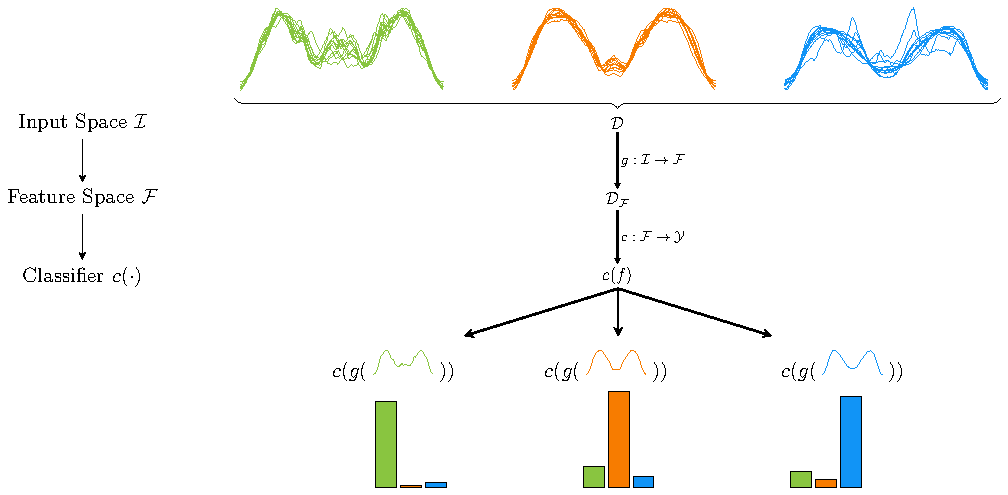
\includegraphics[width=\textwidth]{figures/combines_ts_hist.pdf}}
\only<2>{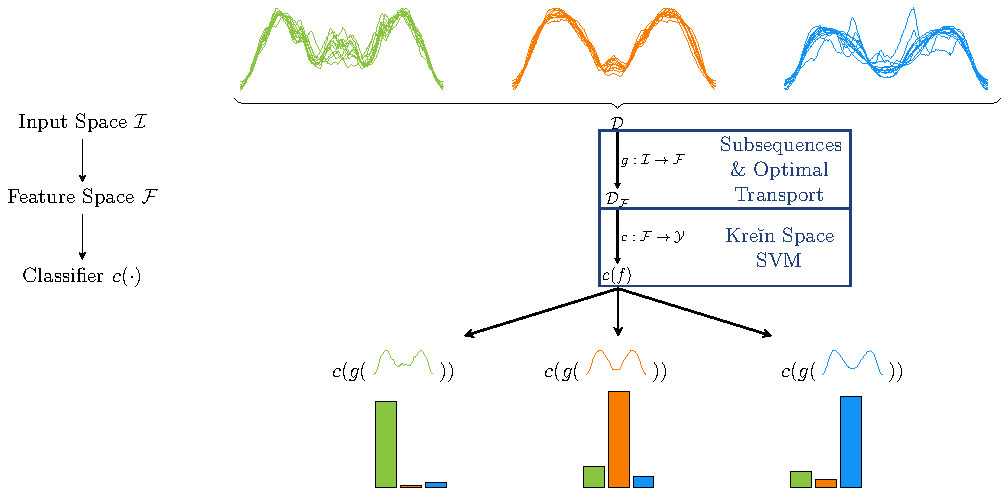
\includegraphics[width=\textwidth]{figures/combines_ts_hist_2.pdf}}
\end{frame}

\section{Feature Space: Subsequences and Optimal Transport}
\begin{frame}{Subsequence Extraction}
	\begin{alertblock}{The Sliding Window Approach}
	\begin{itemize}
		\item Window Size $w$
		\item Stride $s$	
	\end{itemize}
	\centering
	\only<1>{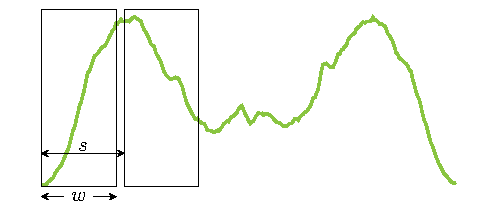
\includegraphics[width=0.8\textwidth]{figures/sliding_window.pdf} \\}
	\only<2>{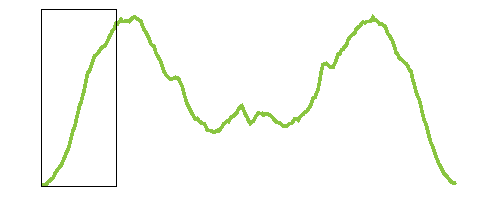
\includegraphics[width=0.8\textwidth]{figures/sliding_window_0.pdf} \\}
	\only<3>{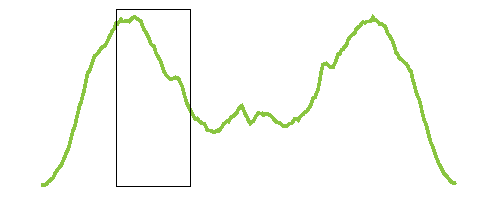
\includegraphics[width=0.8\textwidth]{figures/sliding_window_1.pdf} \\}
	\only<4>{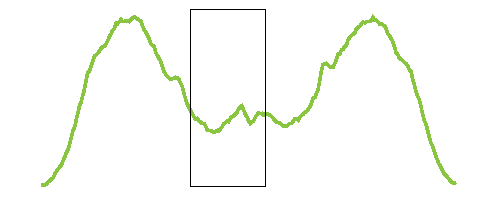
\includegraphics[width=0.8\textwidth]{figures/sliding_window_2.pdf} \\}
	\only<5>{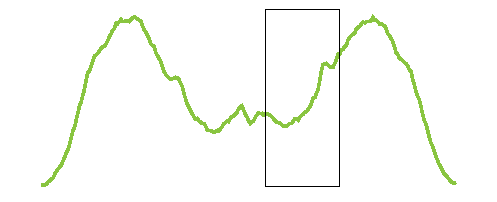
\includegraphics[width=0.8\textwidth]{figures/sliding_window_3.pdf} \\}
	\only<6>{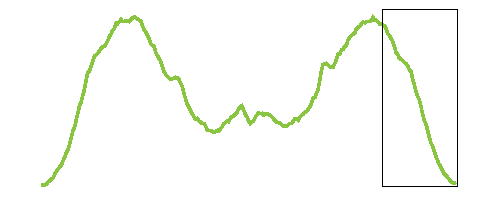
\includegraphics[width=0.8\textwidth]{figures/sliding_window_4.pdf} \\}
	\vspace*{1cm}
	\begin{tikzpicture}
		\only<2-6>{\node[inner sep=0pt] (ts) at (-2,-1)
		{
\includegraphics[height=1.2cm]{figures/subsequences_for_SW_0.pdf}};}
		
		\only<3-6>{\node[inner sep=0pt] (ts) at (-0.5,-1)
		{
\includegraphics[height=1.2cm]{figures/subsequences_for_SW_1.pdf}};}
		
		\only<4-6>{\node[inner sep=0pt] (ts) at (1.5,-1)
		{
\includegraphics[height=1.2cm]{figures/subsequences_for_SW_2.pdf}};}
		
		\only<5-6>{\node[inner sep=0pt] (ts) at (3.5,-1)
		{
\includegraphics[height=1.2cm]{figures/subsequences_for_SW_3.pdf}};}
		
		\only<6>{\node[inner sep=0pt] (ts) at (5.5,-1)
		{
\includegraphics[height=1.2cm]{figures/subsequences_for_SW_4.pdf}};}

	\end{tikzpicture}
\end{alertblock}	
\end{frame}

\begin{frame}{Subsequence Distance Matrix}
	
\documentclass{standalone}
\usepackage[utf8]{inputenc}
\usepackage{pgfplots}
\pgfplotsset{compat=newest}

\usepgfplotslibrary{groupplots}
\definecolor{printable_1}{RGB}{137, 197, 64}
\definecolor{printable_2}{RGB}{247, 124, 0}
\definecolor{printable_3}{RGB}{ 17, 148, 246}
\definecolor{printable_4}{RGB}{103, 52, 186}

\usetikzlibrary{external}
\usetikzlibrary{calc}
\usetikzlibrary{arrows}

\newcommand{\dataset}{ArrowHead}


\begin{document}
    \begin{tikzpicture}
           
           %\node[inner sep=0pt] (hist) at (0,3)
           %{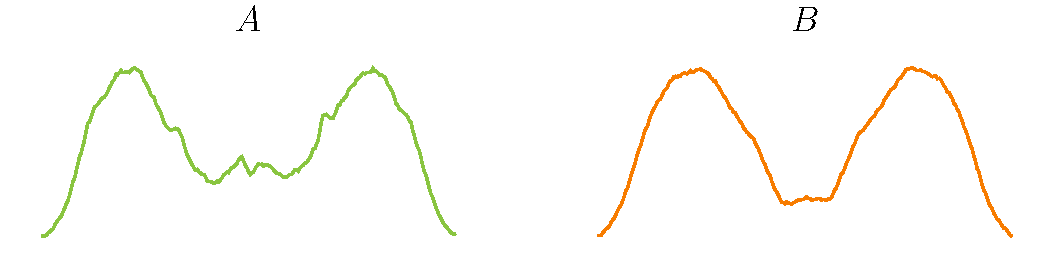
\includegraphics[width=0.8\textwidth]{figures/two_ts.pdf}};
           
           \node[inner sep=0pt] (hist) at (-4.3,-4.3)
           {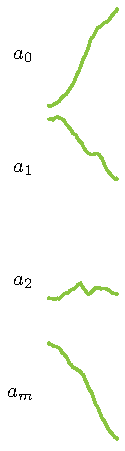
\includegraphics[height=6.5cm]{subsequences_0.pdf}};
           
           \node[inner sep=0pt] (hist) at (0,0)
           {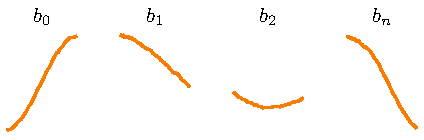
\includegraphics[width=.5\textwidth]{subsequences_1.pdf}};
           
           \node at (0, -4) {\LARGE $D_{u,v} = \sqrt{\sum_{i=0}^{l}(p_{u,i} - q_{v,i})^2}$};
           
    \end{tikzpicture}
\end{document}
\end{frame}

\section{Optimal Transport and the Wasserstein Distance}

\begin{frame}{Optimal Transport}
	\begin{alertblock}{Transportation Theory}
	\begin{itemize}
		\item Study of optimal transportation and allocation of resources
		\item \textbf{Gaspard Monge (1746–1818)} \\ Morph one probability distribution into a second one with minmal cost.
		\item \textbf{Frank Lauren Hitchcock (1875 – 1957)} \\ Transport a commodity from different sources to different ``sinks''.
		\item \textbf{Leonid Kantorovich (1912 - 1986)} \\ Distribute soldiers to the frontline.
	\end{itemize}
\end{alertblock}
\end{frame}

\begin{frame}{The Swiss Kantorovich Problem}
	\only<1>{\includegraphics[width=\textwidth]{figures/kantorovich_0.pdf}}
\only<2>{\includegraphics[width=\textwidth]{figures/kantorovich_1.pdf}}
\only<3>{\includegraphics[width=\textwidth]{figures/kantorovich_2.pdf}}
\only<4>{\includegraphics[width=\textwidth]{figures/kantorovich_3.pdf}}
\end{frame}

\begin{frame}{The Swiss Kantorovich Problem}
	
\documentclass{standalone}
\usepackage[utf8]{inputenc}
\usepackage{pgfplots}
\pgfplotsset{compat=newest}

\usepgfplotslibrary{groupplots}
\definecolor{printable_1}{RGB}{137, 197, 64}
\definecolor{printable_2}{RGB}{247, 124, 0}
\definecolor{printable_3}{RGB}{ 17, 148, 246}
\definecolor{printable_4}{RGB}{103, 52, 186}

\usetikzlibrary{external}
\usepackage{calc}

\definecolor{vispCol}{RGB}{255, 255, 255}
\definecolor{printable_2}{RGB}{247, 124, 0}
\definecolor{printable_3}{RGB}{ 17, 148, 246}
\definecolor{printable_4}{RGB}{103, 52, 186}

\begin{document}
    \begin{tikzpicture}
    	\def\cheeseSize{3cm}
    	\def\hutSize{4cm}
    	
		\node[inner sep=0, opacity=0.7] at (0,0)
		{\includegraphics[width=1834px]{swiss_alps.png}};
    	
    	% Visp
      \node[inner sep=0pt] (visp) at (-13,-11)
    	{
\includegraphics[width=\cheeseSize]{cheese.png}};
	    \node[scale=8, yellow] at ($(visp.east)+(2,0)$) {90};
    	
	    % Raron
    	\node[inner sep=0pt] (raron) at (-25,-6)
    	{
\includegraphics[width=\cheeseSize]{cheese.png}};
    	 \node[scale=8, yellow] at ($(raron.south)+(0,-2)$) {60};
    	
    	% Termen
    	%\node[inner sep=0pt] (termen) at (5, -2)
    	%{
\includegraphics[width=\cheeseSize]{cheese.png}};
    	
    	% Fiesch
    	\node[inner sep=0pt] (fiesch) at (14, 4)
    	{
\includegraphics[width=\cheeseSize]{cheese.png}};
    	\node[scale=8, yellow] at ($(fiesch.east)+(2.5,0)$) {150};
    	
    	
    	% Huts
    	\node[inner sep=0pt] (hut1) at (-19,4)
    	{
\includegraphics[width=\hutSize]{hut.png}};
    	\node[scale=8, black] at ($(hut1.south west)+(-1,-1)$) {120};
    	
    	\node[inner sep=0pt] (hut2) at (-10, 1)
    	{
\includegraphics[width=\hutSize]{hut.png}};
    	\node[scale=8, black] at ($(hut2.north east)+(1,1)$) {90};
    	
    	\node[inner sep=0pt] (hutGrindel) at (-3, 13)
    	{
\includegraphics[width=\hutSize]{hut.png}};
    	\node[scale=8, black] at ($(hutGrindel.east)+(1.5,0)$) {90};
    	
    	% Raron to hut1
    	\draw[line width=3mm, red, dotted] (raron.east) -- ++(5,5) -- ++(1,2) -- (hut1.south);
    	% Raron to hut2
    	\draw[line width=3mm, red, dotted] (raron.east) -- ++(5,-1) -- ++(2,4) -- ++(2,-2) -- (hut2.south);
    	% Raron to grindelwald
    	\draw[line width=3mm, red, dotted] (raron.west) -- ++(-4,4) -- ++(3,4) -- (hutGrindel.south west);
    	
    \end{tikzpicture}
\end{document}
\end{frame}

% \begin{frame}{Wasserstein Distance on Time Series}
%   \centering
%   \begin{columns}
%   \begin{column}{columnwidth=0.33\linewidth}
%   \subcaptionbox{Subsequence distance matrix\label{sfig:Subsequence distance matrix}}{
%     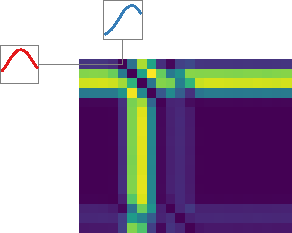
\includegraphics[height=3.0cm, width=3.5cm]{figures/subsequence_distances.pdf}
%   }
%   \end{column}
%   \subcaptionbox{Optimal transport plan\label{sfig:Optimal transport plan}}{%
%     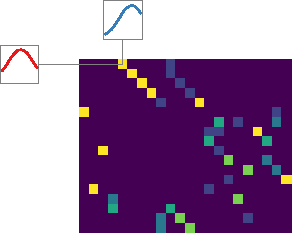
\includegraphics[height=3.0cm, width=3.5cm]{figures/optimal_transport.pdf}
%   }
%   \subcaptionbox{Transport plan visualisation\label{sfig:Intuition transport plan}}
%   {%
%     \begin{tikzpicture}
%       \begin{axis}[%
%         axis lines = none,
%         height     =  4.5cm,
%         width      =  7.0cm,
%       ]
%         \addplot[Set1-A, thick, no marks] table[x=x, y=a, col sep=comma] {./data/overview_TS_uneq_length_1.csv};
%         \addplot[
%           Set1-B, thick, no marks,
%           y filter/.expression = {
%             y - 10
%           },
%         ] table[x=x, y=a, col sep=comma] {./data/overview_TS_2.csv};

%         \draw[draw opacity=0.8, line width=0.6pt] (0.00,0.05) -- (20.00,-10.03);
%         \draw[draw opacity=0.8, line width=0.6pt] (5.00,0.08) -- (25.00,-9.75);
%         \draw[draw opacity=0.8, line width=0.6pt] (10.00,1.38) -- (30.00,-7.66);
%         \draw[draw opacity=0.8, line width=0.6pt] (15.00,3.95) -- (35.00,-6.24);
%         \draw[draw opacity=0.8, line width=0.6pt] (20.00,1.87) -- (60.00,-9.92);
%         \draw[draw opacity=0.8, line width=0.6pt] (25.00,0.15) -- (0.00,-9.98);
%         \draw[draw opacity=0.8, line width=0.15882352941176556pt] (30.00,-0.04) -- (70.00,-10.03);
%         \draw[draw opacity=0.8, line width=0.6pt] (35.00,0.01) -- (90.00,-10.01);
%         \draw[draw opacity=0.8, line width=0.15882352941176434pt] (40.00,-0.01) -- (65.00,-9.98);
%         \draw[draw opacity=0.8, line width=0.6pt] (45.00,-0.00) -- (10.00,-10.01);
%         \draw[draw opacity=0.8, line width=0.30588235294117666pt] (50.00,-0.01) -- (75.00,-9.98);
%         \draw[draw opacity=0.8, line width=0.45294117647058646pt] (55.00,0.00) -- (85.00,-10.01);
%         \draw[draw opacity=0.8, line width=0.6pt] (60.00,-0.00) -- (105.00,-9.99);
%         \draw[draw opacity=0.8, line width=0.6pt] (65.00,-0.01) -- (5.00,-10.03);
%         \draw[draw opacity=0.8, line width=0.4529411764705877pt] (70.00,0.01) -- (80.00,-9.96);
%         \draw[draw opacity=0.8, line width=0.15882352941176434pt] (75.00,0.02) -- (15.00,-9.99);
%         \draw[draw opacity=0.8, line width=0.30588235294117666pt] (80.00,0.38) -- (50.00,-9.60);
%         \draw[draw opacity=0.8, line width=0.30588235294117666pt] (85.00,1.56) -- (55.00,-8.53);
%       \end{axis}
%     \end{tikzpicture}
%   }
%   \end{figure}
%   \end{columns} 
% \end{frame}

\section{A Wasserstein Kernel for Time Series}
	\tikzset{
  invisible/.style={opacity=0},
  transparent/.style={opacity=0.2},
  visible on/.style={alt={#1{}{invisible}}},
  transparent on/.style={alt={#1{transparent}{}}},
  alt/.code args={<#1>#2#3}{%
    \alt<#1>{\pgfkeysalso{#2}}{\pgfkeysalso{#3}} % \pgfkeysalso doesn't change the path
  },
}

% Self arc
\def\centerarc[#1](#2)(#3:#4:#5)% Syntax: [draw options] (center) (initial angle:final angle:radius)
    { \draw[#1] ($(#2)+({#5*cos(#3)},{#5*sin(#3)})$) arc (#3:#4:#5); }

\begin{frame}{Time Series Pairwise Distance Calculation}
    \begin{figure}[t]
  \centering
    \begin{tikzpicture}
      \begin{axis}[%
        axis lines = none,
        height     =  8cm,
        width      =  11.0cm,
      ]
        \addplot[Set1-A, thick, no marks, visible on=<1-5>] table[x=x, y=a, col sep=comma] {./data/overview_TS_uneq_length_1.csv};
        \addplot[
          Set1-B, thick, no marks,
          y filter/.expression = {
            y - 10
          },
          visible on=<2>,
          transparent on=<3-5>
        ] table[x=x, y=a, col sep=comma] {./data/overview_TS_2.csv};
        
        \addplot[
          Set1-B, thick, no marks,
          x filter/.expression = {
            x + 130
          },
          y filter/.expression = {
            y - 10
          },
          visible on=<3>,
          transparent on=<4-5>
        ] table[x=x, y=a, col sep=comma] {./data/overview_TS_3.csv};
        \addplot[
          Set1-B, thick, no marks,
          x filter/.expression = {
            x + 260
          },
          y filter/.expression = {
            y - 10
          },
          visible on=<4>,
          transparent on=<5-5>
        ] table[x=x, y=a, col sep=comma] {./data/overview_TS_3.csv};
        \addplot[
          Set1-B, thick, no marks,
          x filter/.expression = {
            x + 390
          },
          y filter/.expression = {
            y - 10
          },
          visible on=<5>,
        ] table[x=x, y=a, col sep=comma] {./data/overview_TS_2.csv};
        % TODO create new timeseries..
        
        \filldraw[fill=ETHa, draw=ETHa, fill opacity=0.0] (280,112) rectangle (320,128);
        \filldraw<2->[fill=ETHa, draw=ETHa, fill opacity=0.7] (320,112) rectangle (360,128);
        \filldraw<3->[fill=ETHa, draw=ETHa, fill opacity=0.6] (360,112) rectangle (400,128);
        \filldraw<4->[fill=ETHa, draw=ETHa, fill opacity=0.2] (400,112) rectangle (440,128);
        \filldraw<5->[fill=ETHa, draw=ETHa, fill opacity=0.8] (440,112) rectangle (480,128);
        
        \draw<2>[draw opacity=0.8, line width=1pt] (50.00,90.00) -- (50.00,40.);
        \node<1-5> at (200,120) {$\wasserstein_1\left(\oneseries_0, \oneseries_\only<1>{0}\only<2>{1}\only<3>{2}\only<4>{3}\only<5>{4}\right)$};
        \draw<3>[draw opacity=0.8, line width=1pt] (50.00,90.00) -- (180.00,40.);
        \draw<4>[draw opacity=0.8, line width=1pt] (50.00,90.00) -- (310.00,40.);
        \draw<5>[draw opacity=0.8, line width=1pt] (50.00,90.00) -- (440.00,40.);
        % \centerarc[black,thick](10,100)(30:270:10)
        
        % SECOND ROW
        \addplot[
          Set1-B, thick, no marks,
          y filter/.expression = {
            y - 1
          },
          visible on=<6->
        ] table[x=x, y=a, col sep=comma] {./data/overview_TS_2.csv};
        
        \addplot[
          Set1-A, thick, no marks,
          y filter/.expression = {
            y - 10
          },
          visible on=<6>,
          transparent on=<7->
        ] table[x=x, y=a, col sep=comma] {./data/overview_TS_uneq_length_1.csv};
        \addplot[ % Had to copy it twice
          Set1-B, thick, no marks,
          x filter/.expression = {
            x + 130
          },
          y filter/.expression = {
            y - 10
          },
          visible on=<8>,
        ] table[x=x, y=a, col sep=comma] {./data/overview_TS_3.csv};
        \filldraw<6->[fill=ETHa, draw=ETHa, fill opacity=0.7] (280,98) rectangle (320,112);
        \filldraw<7->[fill=ETHa, draw=ETHa, fill opacity=0.0] (320,98) rectangle (360,112);
        \filldraw<8->[fill=ETHa, draw=ETHa, fill opacity=0.4] (360,98) rectangle (400,112);
        
        
        \draw<6>[draw opacity=0.8, line width=1pt] (50.00,70.00) -- (50.00,40.);
        \node at (200,106) {$\wasserstein_1\left(\oneseries_1, \oneseries_\only<6>{0}\only<7>{1}\only<8>{2}\right)$};
        \draw<8>[draw opacity=0.8, line width=1pt] (50.00,70.00) -- (180.00,40.);
        
        
      \end{axis}
    \end{tikzpicture}
  \end{figure}
\end{frame}

\begin{frame}{Wasserstein Distance Matrix}
    \centering
    \LARGE
    % TODO: CREATE PDF WITH MATRIX
    $\mathcal{D} = $\includegraphics[width=0.1\textwidth]{figures/wassmatrix.tex}$ \in \real^{|\allseries|\times |\allseries|}$ \\
    $\mathcal{D}_{ij} = \wasserstein_1\left(\oneseries_i, \oneseries_j\right)
    $
\end{frame}

\begin{frame}{From Distance to Kernels}
  \begin{definition}[Wasserstein time series kernel]
  \normalsize
  Let $\oneseries_i$ and $\oneseries_j$ be two time series, and $\shapelet_{i1}, \dots, \shapelet_{iU}$
  as well as $\shapelet_{j1}, \dots, \shapelet_{jV}$ be their respective
  subsequences. Moreover, let $D$ be a $U \times V$ matrix that contains
  the pairwise distances of all subsequences, such that
  %
  $D_{uv} := \dist\left(\shapelet_{iu}, \shapelet_{jv}\right)$,
  %
  where $\dist(\cdot, \cdot)$ denotes the usual Euclidean distance.
  The optimisation problem
  %
  \begin{equation}\
   \wasserstein_1\left(\oneseries_i, \oneseries_j\right) := \min_{P \in \Gamma\left(\oneseries_i, \oneseries_j\right)} \left\langle D, P \right\rangle_{\mathrm{F}},
    \label{eq:Our distance}
  \end{equation}
  %
  yields the optimal transport cost to transform $\oneseries_i$
  into $\oneseries_j$ by means of their subsequences. Then, given
  $\lambda\in\real_{> 0}$, we can define
  %
  \begin{equation}
    \Method\left(\oneseries_i, \oneseries_j\right) := \exp\left(-\lambda \wasserstein_1\left(\oneseries_i, \oneseries_j\right)\right),
    \label{eq:Our kernel}
  \end{equation}
  %
  which we refer to as our \emph{Wasserstein-based subsequence kernel};
  \end{definition}
\end{frame}

%%%%%%%%%%%%%%%%%%%%%%%%%%%%%%%%%%%%%%%%%%%%%%%%%%%%%%%%%%%%%%%%%%%%%%%%
% Algorithms
%%%%%%%%%%%%%%%%%%%%%%%%%%%%%%%%%%%%%%%%%%%%%%%%%%%%%%%%%%%%%%%%%%%%%%%%

\definecolor{mydarkblue}{rgb}{0,0.08,0.45}

\renewcommand{\algorithmicrequire}{\textbf{Input:}}
\renewcommand{\algorithmicensure}{\textbf{Output:}}
\renewcommand{\algorithmiccomment}[1]{\qquad \textcolor{ETHf}{//} \textcolor{ETHf}{#1}}

\begin{frame}{\longmethod}
    \begin{algorithm}[H]
      \footnotesize
      \caption{\longmethod}
      \begin{algorithmic}[1]
        \REQUIRE{Time series for training and testing
        $\allseries_{\text{train}}$, $\allseries_{\text{test}}$; subsequence
        length $w$; kernel weight factor $\lambda$}
        \ENSURE{$\mathcal{K}^{\,\text{train}}, \mathcal{K}^{\,\text{test}}$}
          \STATE $\shapelets^{\text{train}} \gets \textsc{Subsequences}({\allseries_{\text{train}}, w})$  \COMMENT{Extract subsequences}
          \STATE $\shapelets^{\text{test}} \gets \textsc{Subsequences}({\allseries_{\text{test}}, w})$ \COMMENT{Extract subsequences}
          \FOR{$\oneseries_i \in \allseries_{\text{train}}$}
            \FOR{$\oneseries_j \in \allseries_{\text{train}}$}
              \STATE $\mathcal{D}_{ij}^{\text{train}} \gets \wasserstein_1\left(\shapelets_i^{\text{train}}, \shapelets_j^{\text{train}}\right)$ \COMMENT{Wasserstein distance calculation (train)} %\Comment{Compute Wasserstein distance between TS using subsequences}
            \ENDFOR
          \FOR{$\oneseries_k \in \allseries_{\text{test}}$}
            \STATE $\mathcal{D}_{ik}^{\text{test}} \gets \wasserstein_1\left(\shapelets_i^{\text{train}}, \shapelets_k^{\text{test}}\right)$ \COMMENT{Wasserstein distance calculation (test)} %\Comment{Compute Wasserstein distance between TS using subsequences}
            \ENDFOR
          \ENDFOR
          \STATE $\mathcal{K}^{\,\text{train}} \gets \exp\left(-\lambda \mathcal{D}^{\text{train}} \right)$ \COMMENT{Kernel matrix calculation}
          \STATE $\mathcal{K}^{\,\text{test}} \gets \exp\left(-\lambda \mathcal{D}^{\text{test}} \right)$ \COMMENT{Kernel matrix calculation}
          \RETURN $\mathcal{K}^{\,\text{train}}, \mathcal{K}^{\,\text{test}}$
      \end{algorithmic}
    \end{algorithm}
\end{frame}

\section{Results}
\begin{frame}{Experiments}
      \begin{description}[%
        labelwidth=\widthof{Comparison}
        ]
        \item[Datasets] \textit{UCR Time Series Archive} \\85 datasets \\ predetermined train/test splits 
        \item[Hyperparameters] 
            Selected via a $5$-fold cross-validation on the training set
        % I don't mention anything about Krein SVM here for simplicity
        \item[Evaluation metric] 
            Classification accuracy
        \item[Comparison partners] 
            \begin{itemize}
                \item[--] Other kernels
                \item[--] DTW-1NN
                \item[--] State-of-the-art methods
            \end{itemize}
        \end{description}
\end{frame}

\begin{frame}{Comparison with Other Kernels}
\begin{figure}[tbp]
  \centering
  {%
    \begin{tikzpicture}[baseline, scale=0.95]
      \begin{axis}[%
        axis x line*  = bottom,
        axis y line*  = left,
        %
        mark size     = 3.0pt,
        xmin          = 0,
        xmax          = 1,
        ymin          = 0,
        ymax          = 1,
        %
        ylabel        = {$\Method{}$},  % TODO
        xlabel        = {Other kernel}, % TODO
        xtick align   = outside,
        ytick align   = outside,
        %
        %
        unit vector ratio*= 1 1 1,
        %
        legend pos     = south east,
        legend style   = {
          font              = \scriptsize,
          draw              = none,
          legend cell align = left,
          fill              = none,
        },
      ]
        \addplot[Dark2-A, only marks, mark=+] table[%
          x       = custom_rbf_kernel_SVM,
          y       = krein_wasserstein_SVM,
          col sep = comma,
        ] {data/computed_accuracies_with_baselines_new.csv};

        \addplot[Dark2-B, only marks, mark=x] table[%
          x       = linear_kernel_SVM,
          y       = krein_wasserstein_SVM,
          col sep = comma,
        ] {data/computed_accuracies_with_baselines_new.csv};

        %\addplot[Dark2-C, only marks, mark=o] table[%
        %  x       = brownian_bridge_SVM,
        %  y       = wasserstein_SVM,
        %  col sep = comma,
        %] {data/computed_accuracies_with_baselines.csv};
        %\legend{RBF, Linear, Brownian bridge}
        \legend{RBF, Linear}

        \node[anchor=west, align=left, font=\small] at (0.40, 0.35) {%
            The other kernel is better\\
            in this region
        };

        \node[anchor=west, align=left, font=\small] at (0.00, 0.90) {%
            $\Method{}$ is better\\
            in this region
        };
        % Diagonal
        \addplot[black] {x};
      \end{axis}
    \end{tikzpicture}%
  }
\end{figure}
\end{frame}

\begin{frame}{Critical Difference Plot}
    The classification performances of methods sharing horizontal bars are not significantly different.
    \begin{figure}
    % TODO: need to obtain the script to generate CD plot
      \centering
      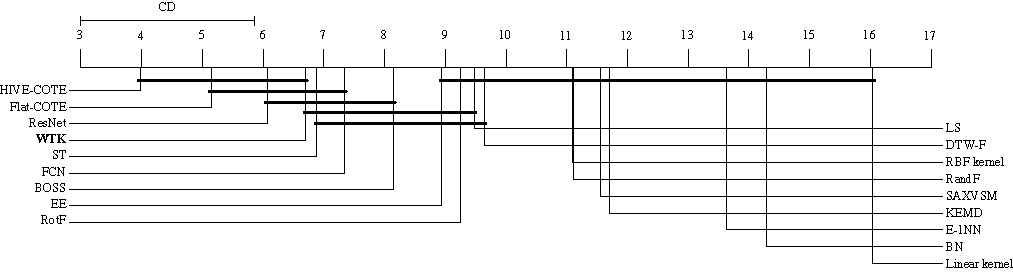
\includegraphics[width=\linewidth]{figures/CD_new.pdf}
    %   \caption{
    %     Critical difference plot, comparing our method~(shown in bold)
    %     with several other methods. The scale indicates the average rank of each method in terms of test accuracy for all data sets. The classification performances of methods sharing horizontal bars are not significantly different. We observe that there is no
    %     statistically significant difference between the performance of our
    %     method and state-of-the-art ensemble methods.
    %   }
    \end{figure}
\end{frame}

\section{Take aways}



\begin{frame}[standout]
  Questions?
\end{frame}

\begin{frame}[allowframebreaks]{References}

  \bibliography{ref}
  \bibliographystyle{abbrvnat}

\end{frame}

\appendix

\end{document}

